Embora o sistema uEye ainda não esteja totalmente operacional, os resultados até o momento evidenciam seu potencial para otimizar a análise preditiva de modelos de UX de alta fidelidade por meio do rastreamento ocular. Testes iniciais serão realizados com as interfaces dos projetos integradores da Fatec, onde alunos participarão ativamente da avaliação, gerando dados que irão alimentar a IA. Em uma fase posterior, a inclusão de clientes finais proporcionará uma coleta de feedback valiosa, permitindo a melhoria contínua do sistema. Os designers poderão consultar a IA para análises ou permitir que os clientes realizem suas próprias avaliações, estabelecendo um ciclo de retroalimentação que impulsionará o desenvolvimento de interfaces mais eficazes.

Apesar de ainda não existir resultados conclusivos, a matriz de rastreamento ocular, que mede a intensidade de atenção dos usuários, promete ser um recurso valioso para a criação de heatmaps que indiquem a eficácia das interfaces.\newline

\subsection*{REASTREAMENTO OCULAR EM JAVA}
A seguir, o protótipo apresentado na imagem demonstra o funcionamento do sistema de rastreamento ocular desenvolvido em Java, utilizando a biblioteca OpenCV. A tela exibida representa a captura em tempo real da câmera do computador do usuário, com sobreposições visuais geradas pelo sistema para identificar a área do rosto e as pupilas.

O sistema realiza a detecção facial ao delimitar o rosto do usuário com um retângulo, enquanto círculos sobre as pupilas indicam o rastreamento preciso da direção do olhar.

\begin{figure}[H]
    \centering
    \caption{Prototipo em Java}%
    \label{fig:pg-telaJava1}
    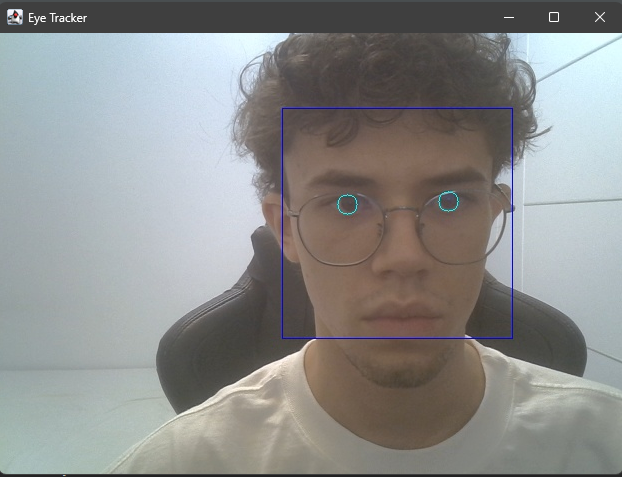
\includegraphics[width=0.72\linewidth]{Illustrations/java1.png}
    \SourceOrNote{Autoria Própria (2024)}
\end{figure}

\subsection*{REASTREAMENTO OCULAR EM PYTHON}
A seguir, é apresentado o funcionamento das telas do sistema de rastreamento ocular, desenvolvido utilizando Python, OpenCV e MediaPipe. As telas exibidas fazem parte da interface interativa destinada ao cliente do designer, que participará do teste avaliando uma interface ou design específico.

O objetivo dessas telas é oferecer uma experiência intuitiva para o cliente enquanto capturam dados precisos sobre os movimentos oculares. Esses dados serão posteriormente processados para gerar heatmaps e outras análises, que servirão como insumos para aprimorar a usabilidade e eficiência dos designs avaliados.

A figura a seguir ilustra a primeira tela apresentada ao cliente. Nela, é exibido um exemplo do design ou interface que está sendo analisado pelo usuário.

\begin{figure}[H]
    \centering
    \caption{Tela 1 - Rastreamento ocular}%
    \label{fig:pg-telaPython1}
    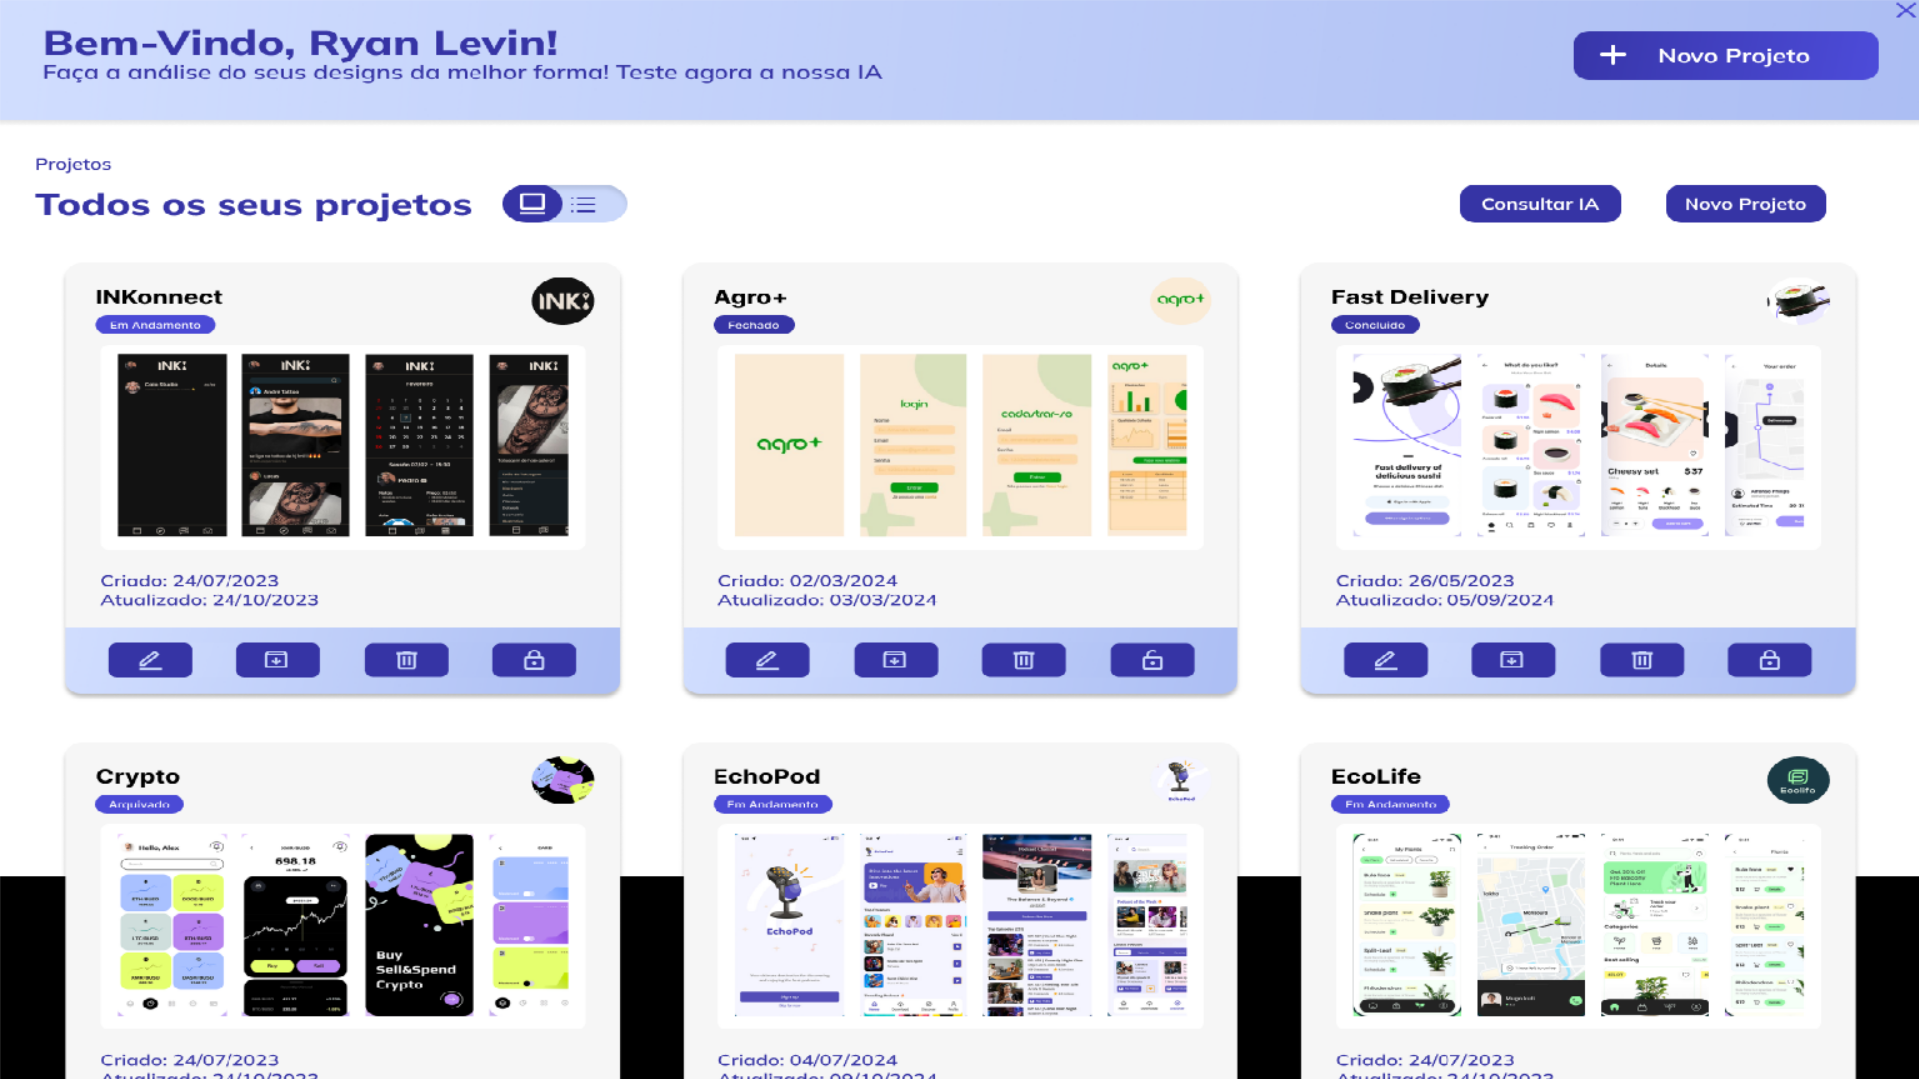
\includegraphics[width=0.72\linewidth]{Illustrations/python1.png}
    \SourceOrNote{Autoria Própria (2024)}
\end{figure}

A próxima figura apresenta o heatmap gerado após o processo de rastreamento ocular sobre a tela mencionada.

\begin{figure}[H]
    \centering
    \caption{Tela 2 - heatmap}%
    \label{fig:pg-telaPython2}
    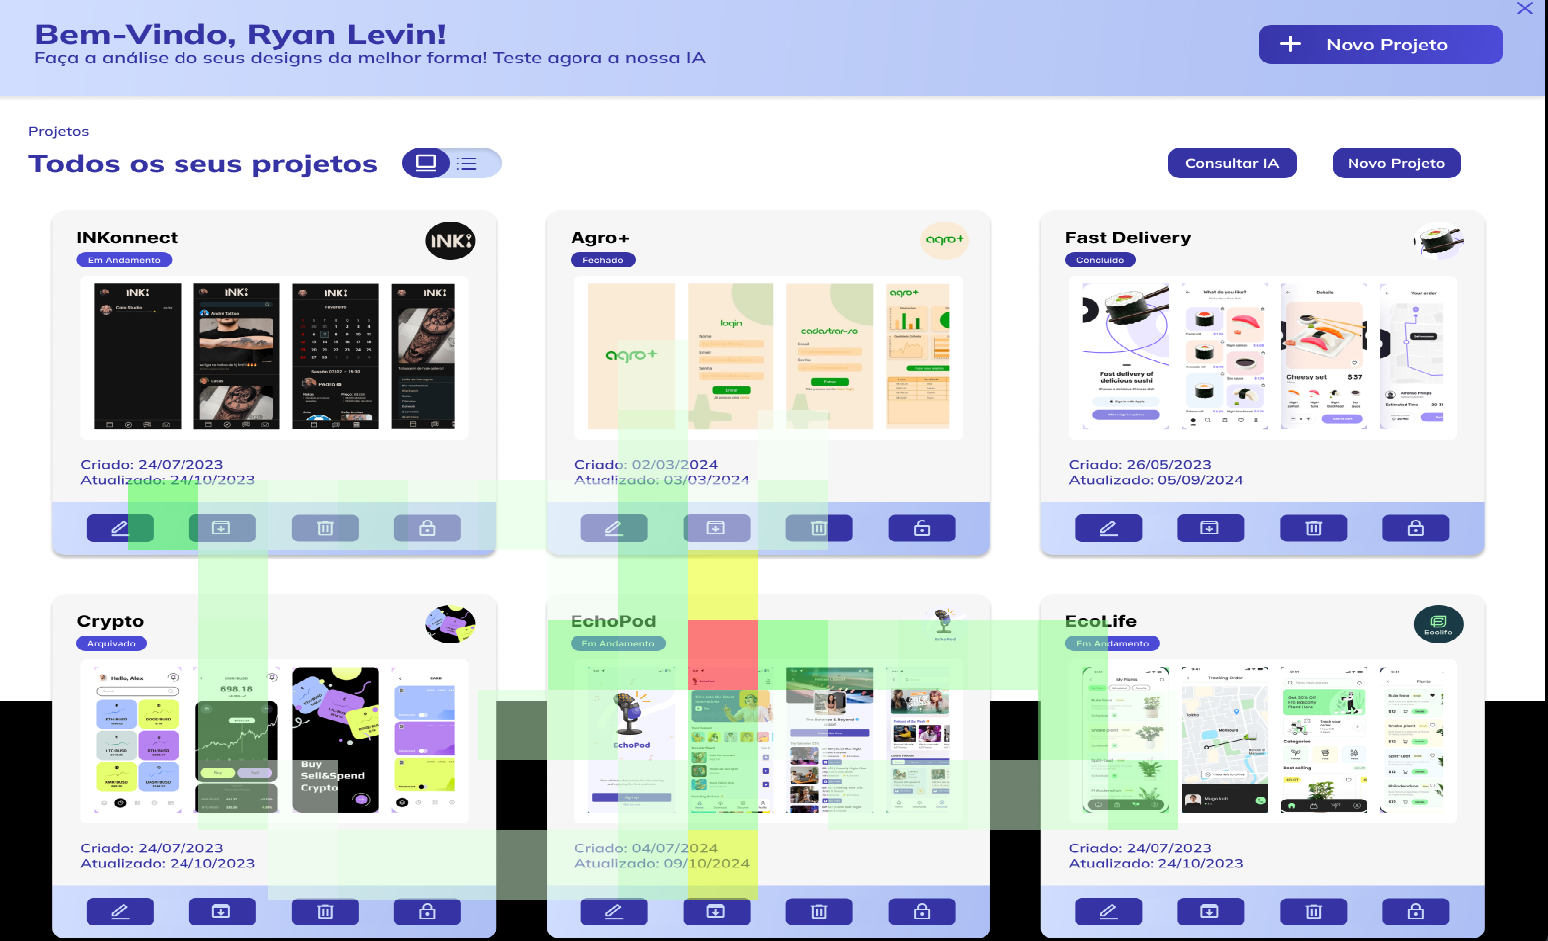
\includegraphics[width=0.72\linewidth]{Illustrations/python2.png}
    \SourceOrNote{Autoria Própria (2024)}
\end{figure}

\subsection*{DIAGRAMA DE CLASSES}
O diagrama de classes é uma representação visual da estrutura de um sistema, descrevendo classes, seus atributos, métodos e os relacionamentos entre elas. Usado principalmente no desenvolvimento orientado a objetos, ele facilita o planejamento e a organização do código ao ilustrar como os componentes interagem, mostrando herança, associações e dependências. Essa visualização ajuda desenvolvedores e analistas a compreender melhor a arquitetura do sistema, promovendo um design mais claro e coeso. \textcite{Lucidchart}

No estudo do projeto, foram identificadas sete classes principais. Primeiramente, as classes Designer e Cliente representam os usuários envolvidos no sistema. O designer, proprietário do projeto, é responsável por iniciar um teste, consultar a IA e visualizar o feedback do cliente. Já o cliente, que adquiriu o serviço do designer, utiliza a interface para avaliar a eficiência do design e fornecer feedback, dados que alimentam a IA.

Para estruturar o projeto e suas análises, foram criadas as classes Projeto e Tela. A classe Tela representa as interfaces específicas que serão analisadas individualmente, em vez do projeto como um todo, no caso da IA.

Uma classe essencial é a de Teste Eye Tracking, que permite a coleta dos dados da matriz de foco visual. A partir dessa classe, surgem as classes de Formulário e Mapa de Calor. O formulário registra a satisfação do cliente após o teste, fornecendo dados para a IA, enquanto a classe Mapa de Calor armazena os dados do Eye Tracking, permitindo que UX designers visualizem os pontos de atenção dos usuários e aperfeiçoem o processo de criação das telas.\newline

\begin{figure}[H]
    \centering
    \caption{Diagrama de Classes}%
    \label{fig:pg-classes}
    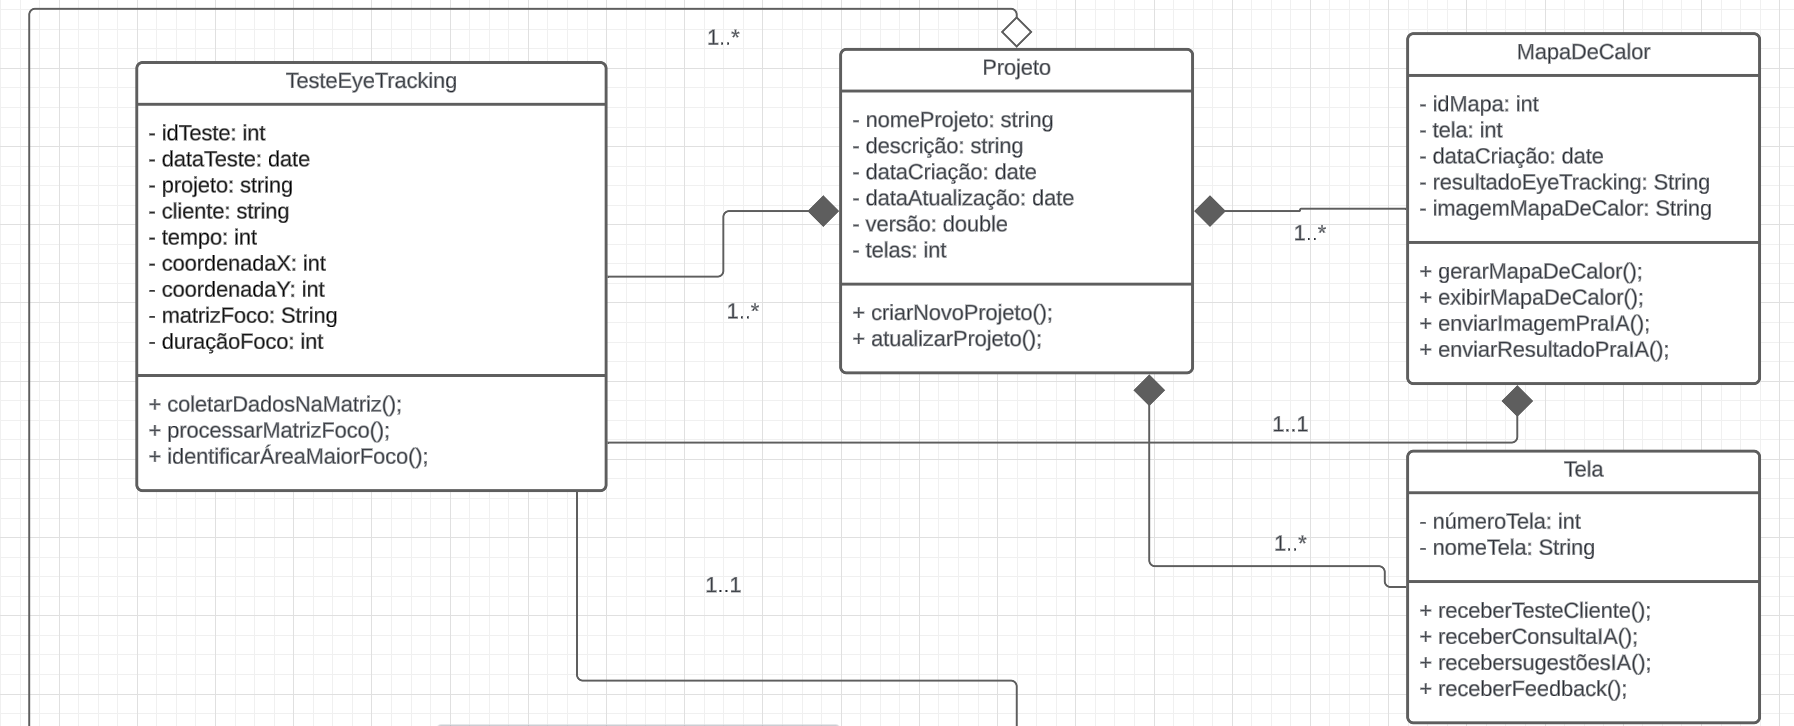
\includegraphics[width=0.72\linewidth]{Illustrations/classes1.png}
    \SourceOrNote{Autoria Própria (2024)}
\end{figure}

\vspace{12pt}

\begin{figure}[H]
    \centering
    \caption{Diagrama de Classes - Continuação}%
    \label{fig:pg-classes2}
    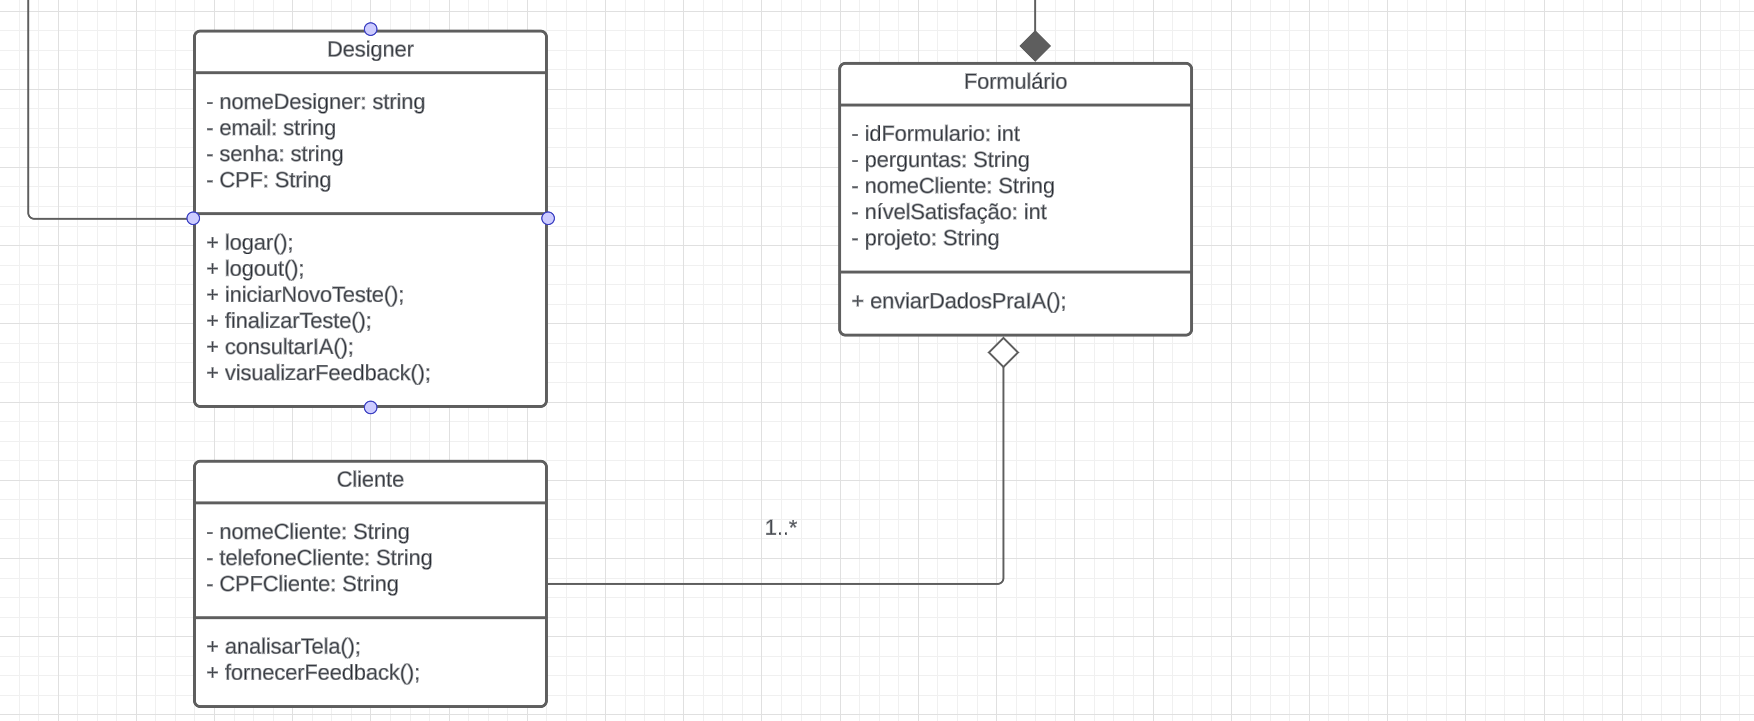
\includegraphics[width=0.72\linewidth]{Illustrations/classes2.png}
    \SourceOrNote{Autoria Própria (2024)}
\end{figure}

\subsection*{DIAGRAMA DE OBJETOS}
O diagrama de objetos é uma representação visual que exibe instâncias específicas de classes em um momento particular do sistema, mostrando objetos com seus valores atuais de atributos e as relações entre eles. Diferente do diagrama de classes, que é mais abstrato e define a estrutura geral, o diagrama de objetos detalha uma visão concreta do estado do sistema em determinado instante, facilitando a compreensão das interações entre os objetos e a verificação de como o sistema se comporta na prática.

No diagrama de objetos, as sete instâncias identificadas representam os principais componentes do sistema e como eles interagem em um cenário específico. A instância designer: Designer contém os dados do designer responsável pelo projeto, incluindo nome, e-mail e CPF, enquanto cli: Cliente apresenta as informações do cliente que está avaliando o projeto.

A instância proj: Projeto refere-se ao projeto sendo analisado, com atributos como nome, descrição, data de criação e atualização, e número de telas. Cada tela é representada por uma instância específica, como tela: Tela, que armazena informações detalhadas sobre uma interface específica do projeto.

O teste: TesteEyeTracking registra os dados coletados pelo Eye Tracking, como a matriz de foco e a duração, facilitando a análise do comportamento do usuário. A partir do teste, temos as instâncias form: Formulário e mapa: MapaDeCalor, onde o formulário coleta o feedback do cliente, e o mapa de calor armazena os dados de visualização, oferecendo insights para os UX designers.\newline

\begin{figure}[H]
    \centering
    \caption{Diagrama de Objetos}%
    \label{fig:pg-objetos}
    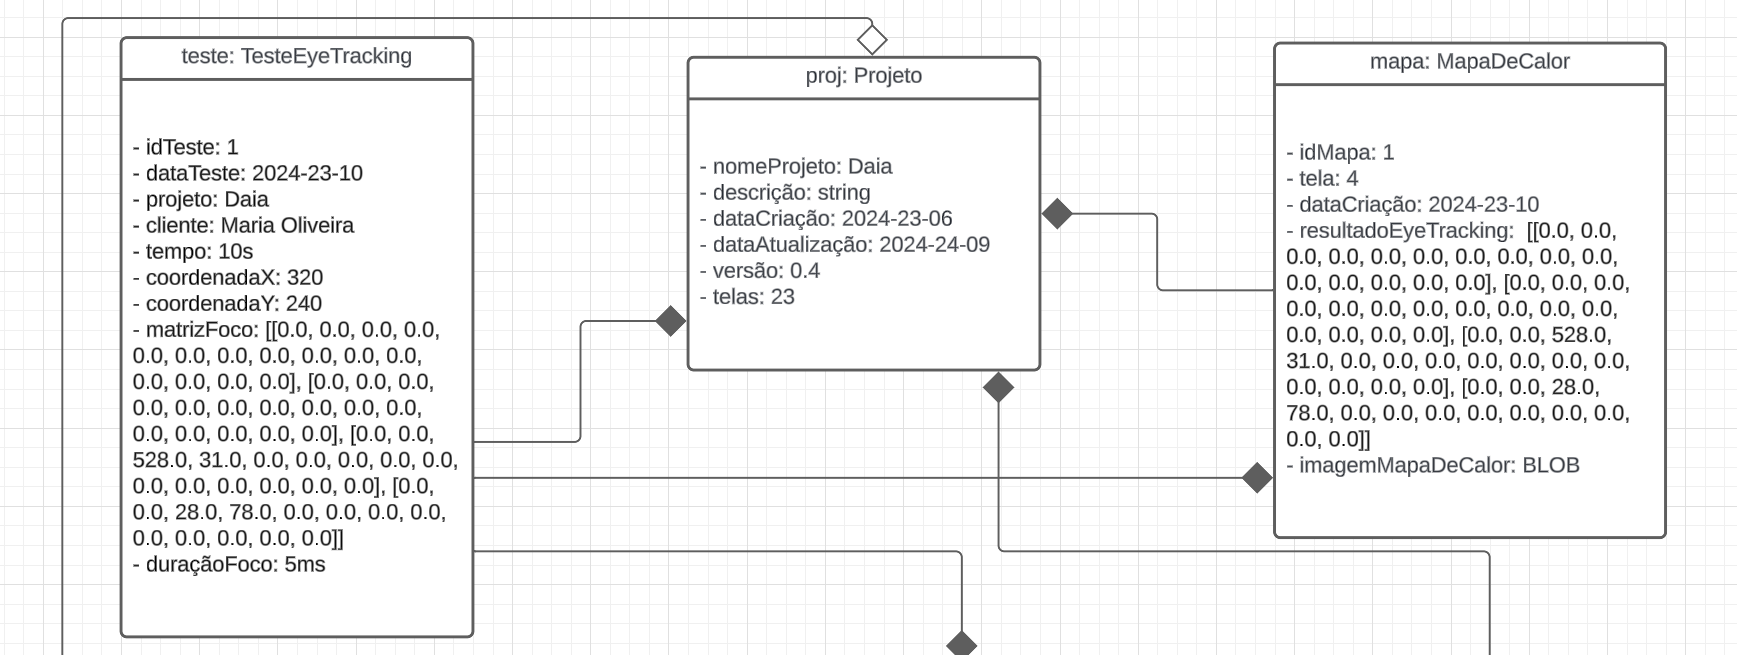
\includegraphics[width=0.72\linewidth]{Illustrations/objetos1.png}
    \SourceOrNote{Autoria Própria (2024)}
\end{figure}

\vspace{12pt}

\begin{figure}[H]
    \centering
    \caption{Diagrama de Objetos - Continuação}%
    \label{fig:pg-objetos2}
    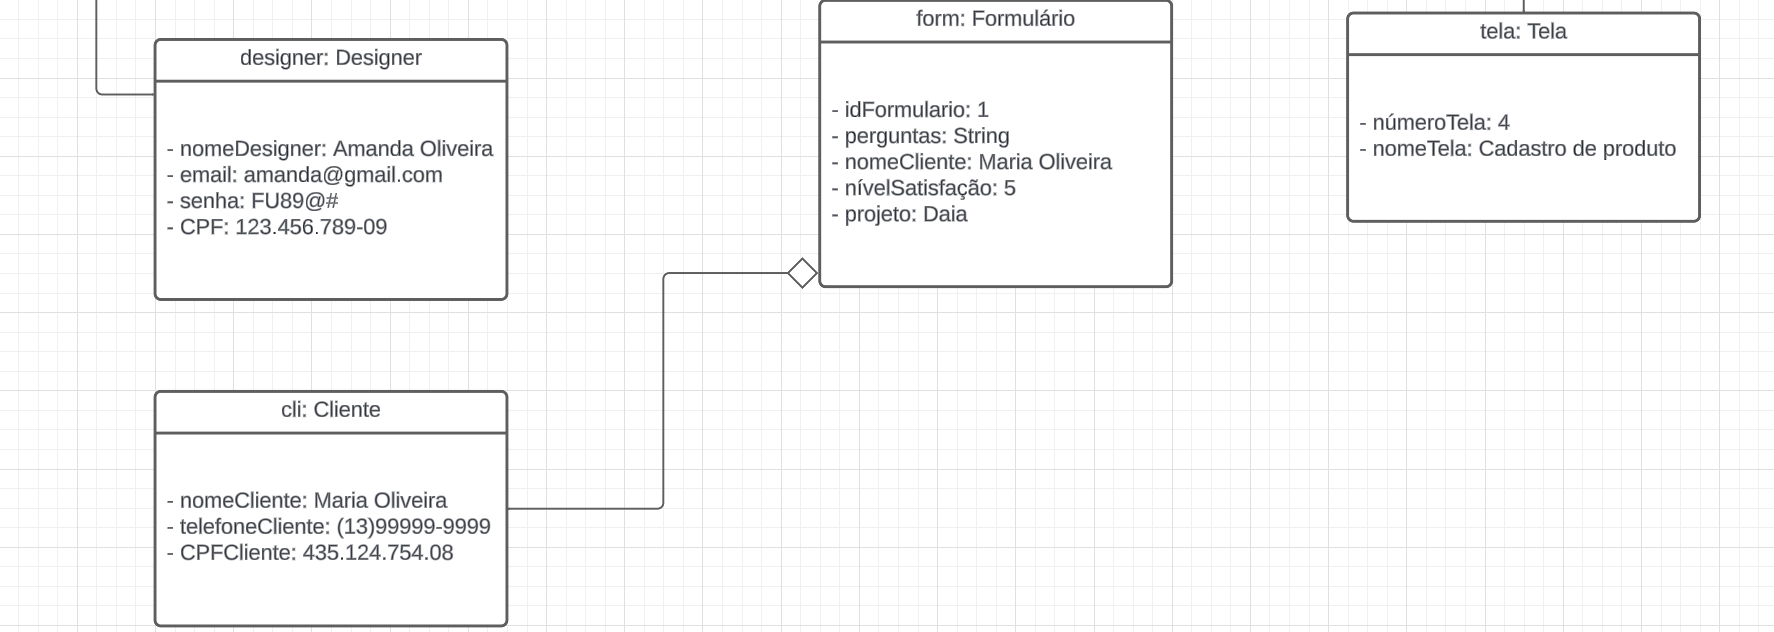
\includegraphics[width=0.72\linewidth]{Illustrations/objetos2.png}
    \SourceOrNote{Autoria Própria (2024)}
\end{figure}

\subsection*{BANCO DE DADOS RELACIONAL}
Para construir o modelo físico do banco de dados da aplicação foi utilizada a Linguagem de Consulta Estruturada (SQL) e o MySQL.

A SQL é uma linguagem de programação padronizada usada para gerenciar e manipular dados em bancos de dados relacionais, organizando informações em tabelas de linhas e colunas. Por meio de comandos SQL, é possível inserir, atualizar, excluir e consultar dados no banco, além de realizar otimizações para melhorar seu desempenho.

O MySQL, por sua vez, é um sistema de gerenciamento de banco de dados relacional de código aberto, mantido pela Oracle, que utiliza a SQL como base para suas operações. É amplamente usado em aplicações web e pode ser instalado em sistemas operacionais diversos, assim como em servidores de nuvem. \textcite{Amazon}\newline

\subsection*{PROTOTIPAÇÃO DO SOFTWARE uEye}
A (\Cref{fig:pg-tela1}) representa a tela inicial do designer. Logo após fazer o login, o mesmo tem acesso a todos os seus projetos podendo decidir qual manipular.

\begin{figure}[H]
    \centering
    \caption{Tela 1 - Tela inicial}%
    \label{fig:pg-tela1}
    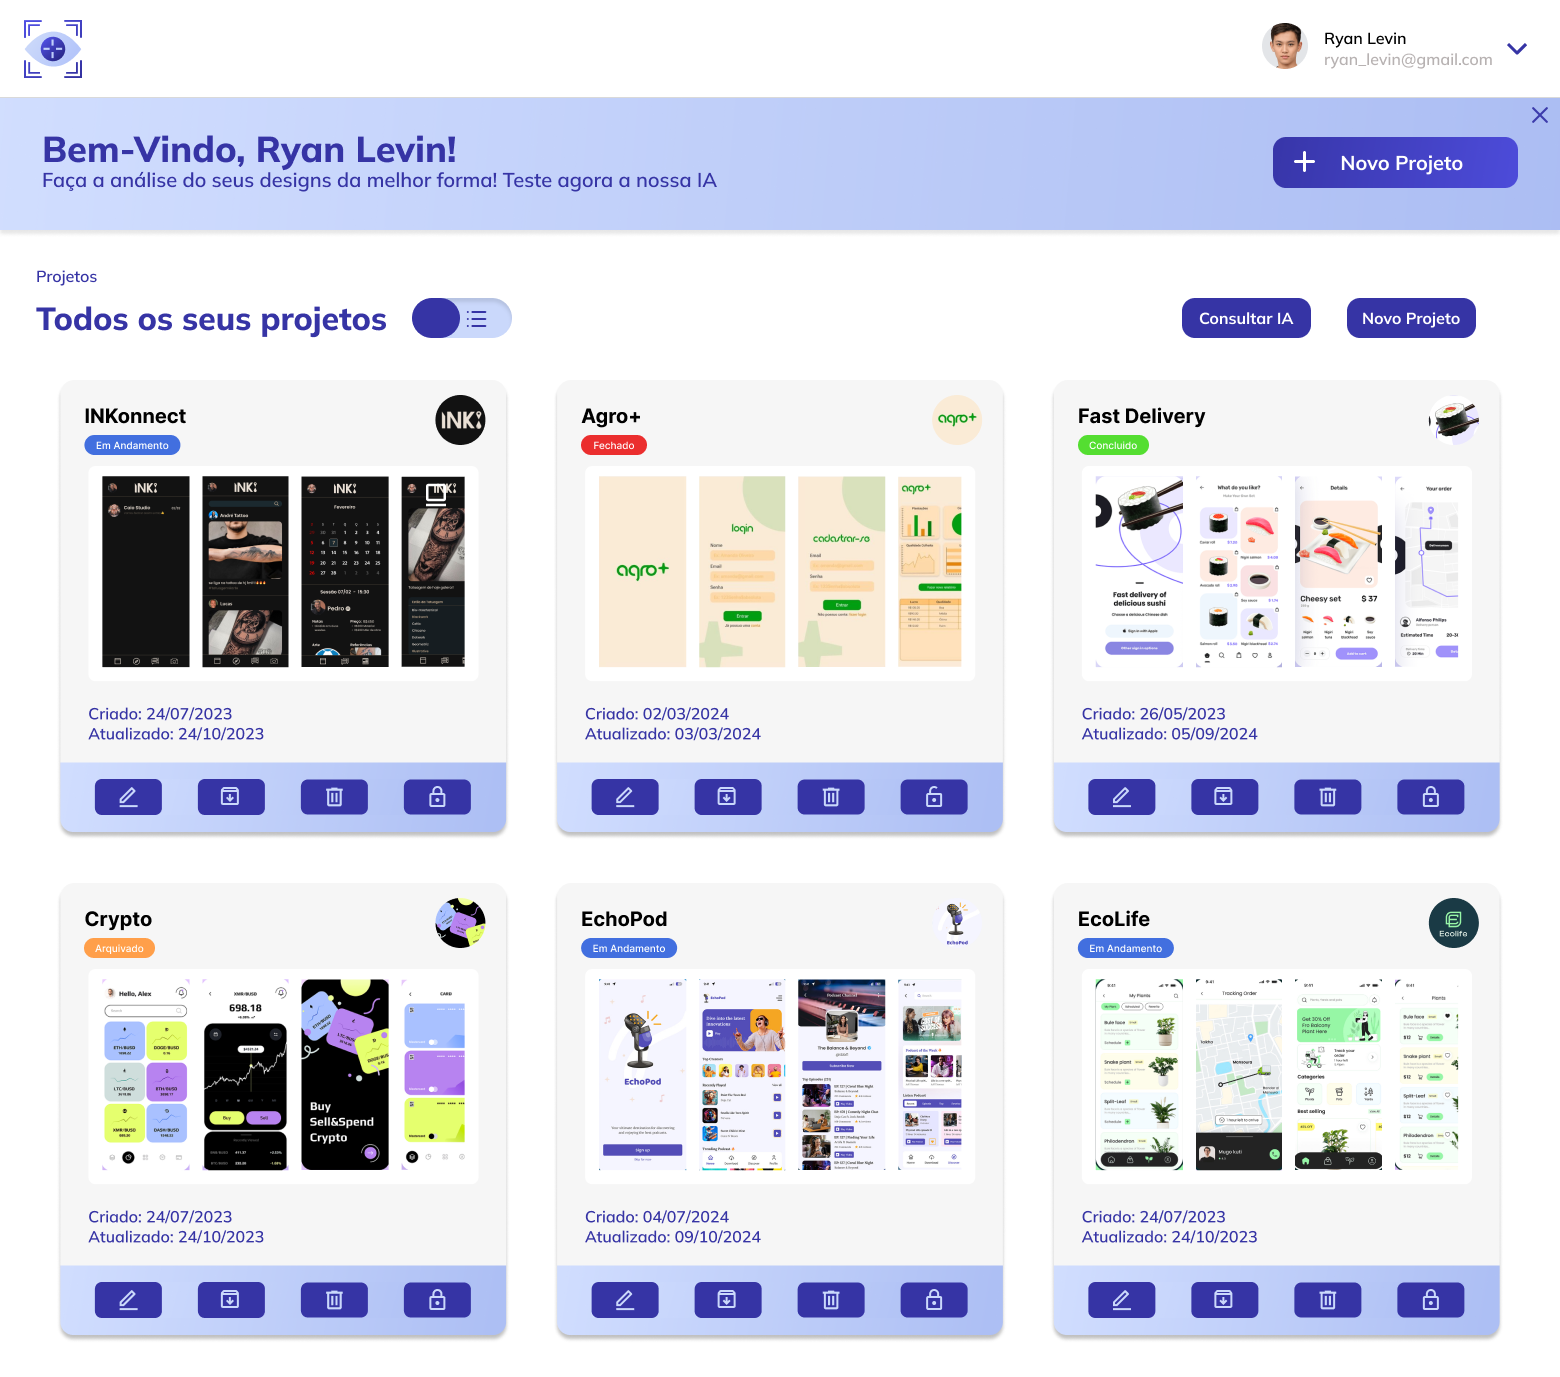
\includegraphics[width=0.72\linewidth]{Illustrations/tela1.png}
    \SourceOrNote{Autoria Própria (2024)}
\end{figure}

A (\Cref{fig:pg-tela2}) representa a tela que o designer tem acesso ao entrar em um projeto. Nela é possível visualizar as telas pertencentes ao projeto, assim como dois gráficos. O da esquerda representa o número de notas baixas atribuídas a esse projeto de acordo com três quesitos. Por exemplo, o projeto em específico obteve trinta e cinco notas baixas no quesito “Atratividade visual”. Enquanto o gráfico da direita ilustra a taxa de satisfação por avaliação através da IA por períodos de tempo, nesse caso, dias. Além disso é possível clicar nos botões de “Consultar IA” e no de “Eye-tracking”, onde no último é possível escolher entre fazer um novo teste ou visualizar as avaliações anteriores de clientes.

\begin{figure}[H]
    \centering
    \caption{Tela 2 - Manipulação do projeto}%
    \label{fig:pg-tela2}
    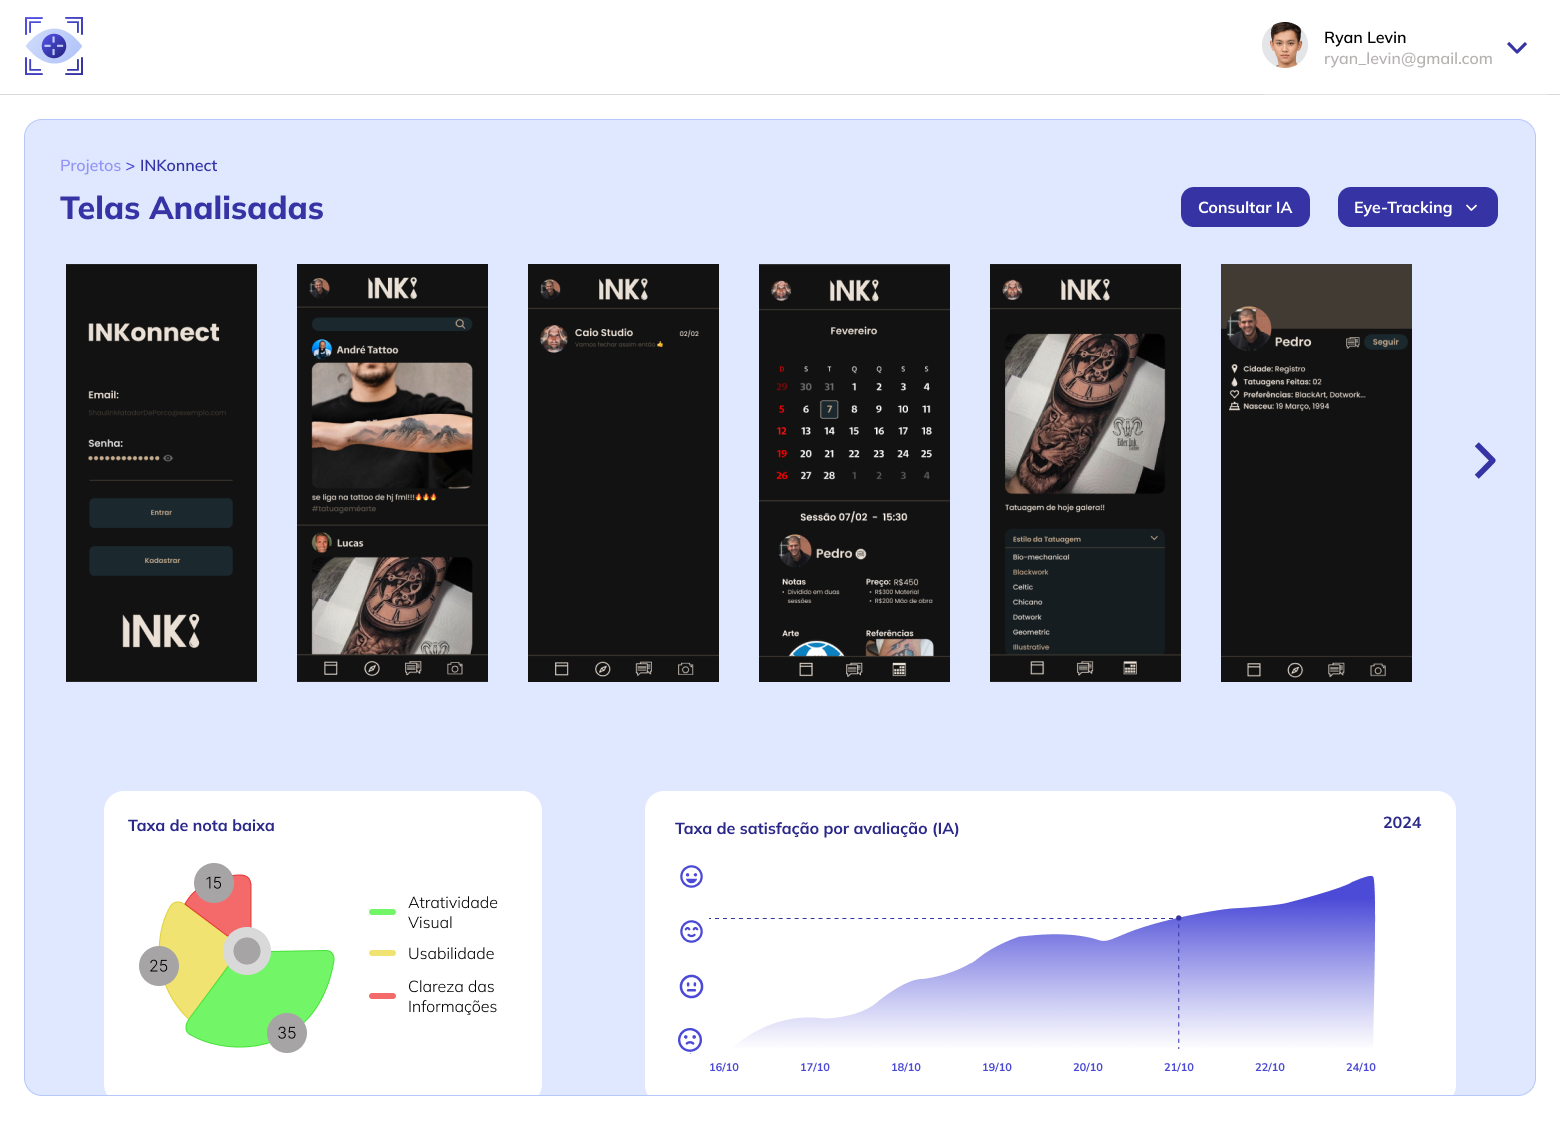
\includegraphics[width=0.72\linewidth]{Illustrations/tela2.png}
    \SourceOrNote{Autoria Própria (2024)}
\end{figure}

Na (\Cref{fig:pg-tela3}), observa-se que, ao clicar em uma das telas do projeto, o usuário pode acessar o histórico de avaliações realizadas pela IA.

\begin{figure}[H]
    \centering
    \caption{Tela 3 - Histórico de avaliações da IA}%
    \label{fig:pg-tela3}
    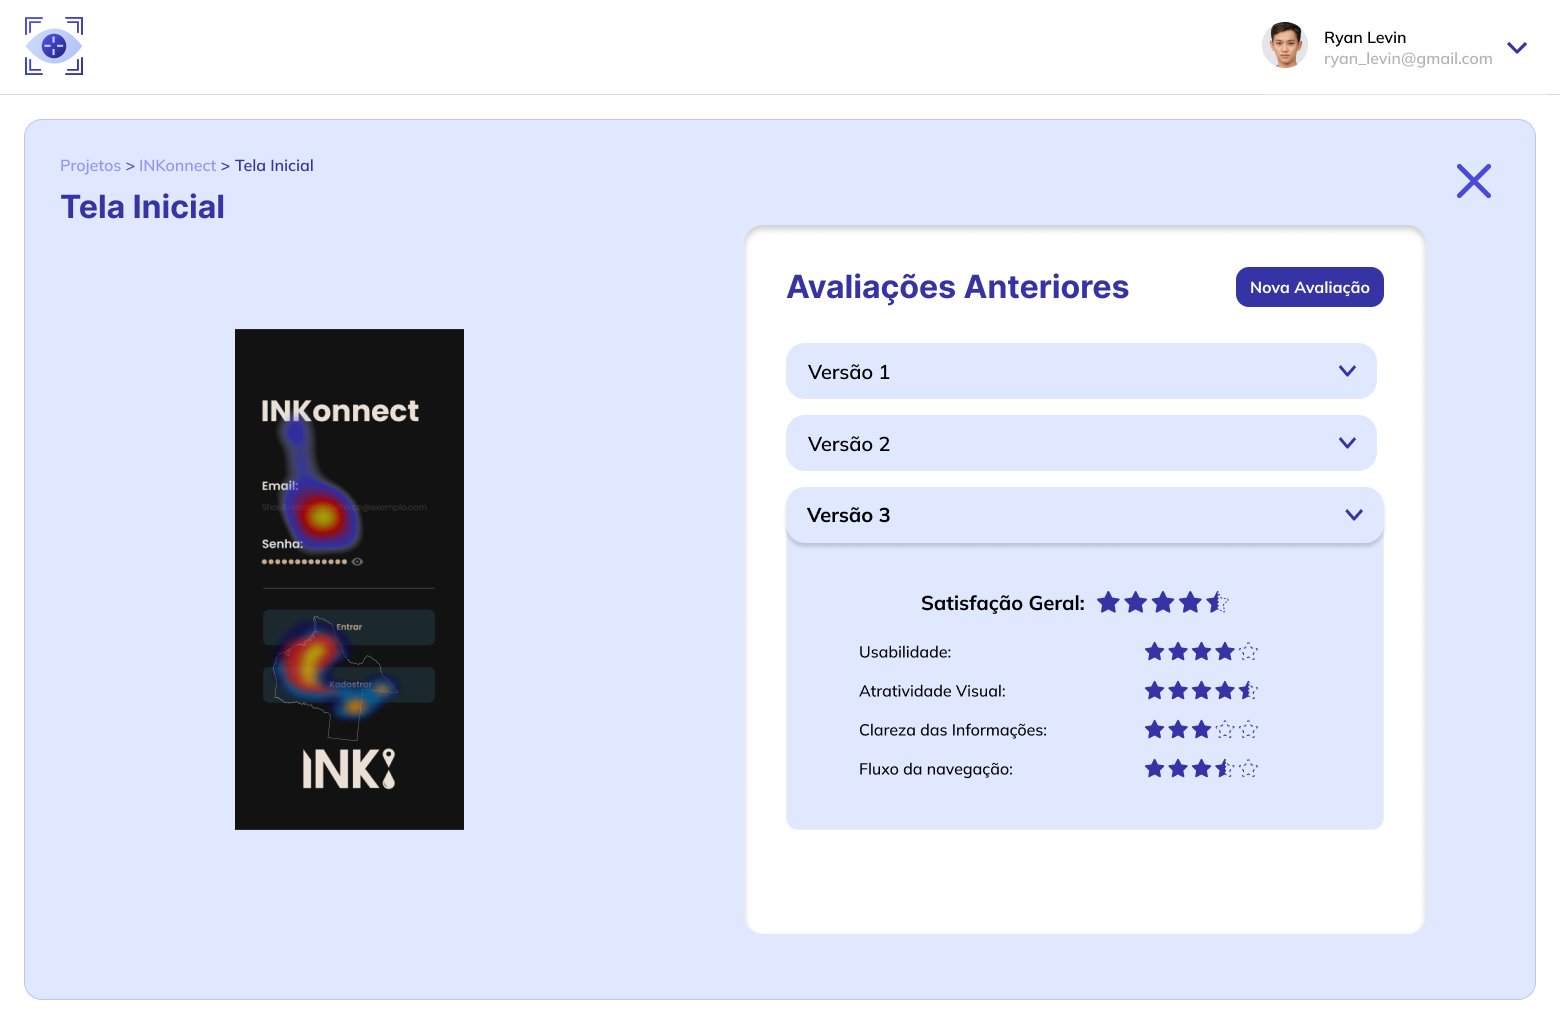
\includegraphics[width=0.72\linewidth]{Illustrations/tela3.png}
    \SourceOrNote{Autoria Própria (2024)}
\end{figure}

Ao clicar no botão “Consultar IA” da \Cref{fig:pg-tela2}, o designer tem acesso à janela (\Cref{fig:pg-tela4}) em que é possível carregar uma tela do projeto para que a IA faça a avaliação da mesma.

\begin{figure}[H]
    \centering
    \caption{Tela 4- Consulta IA}%
    \label{fig:pg-tela4}
    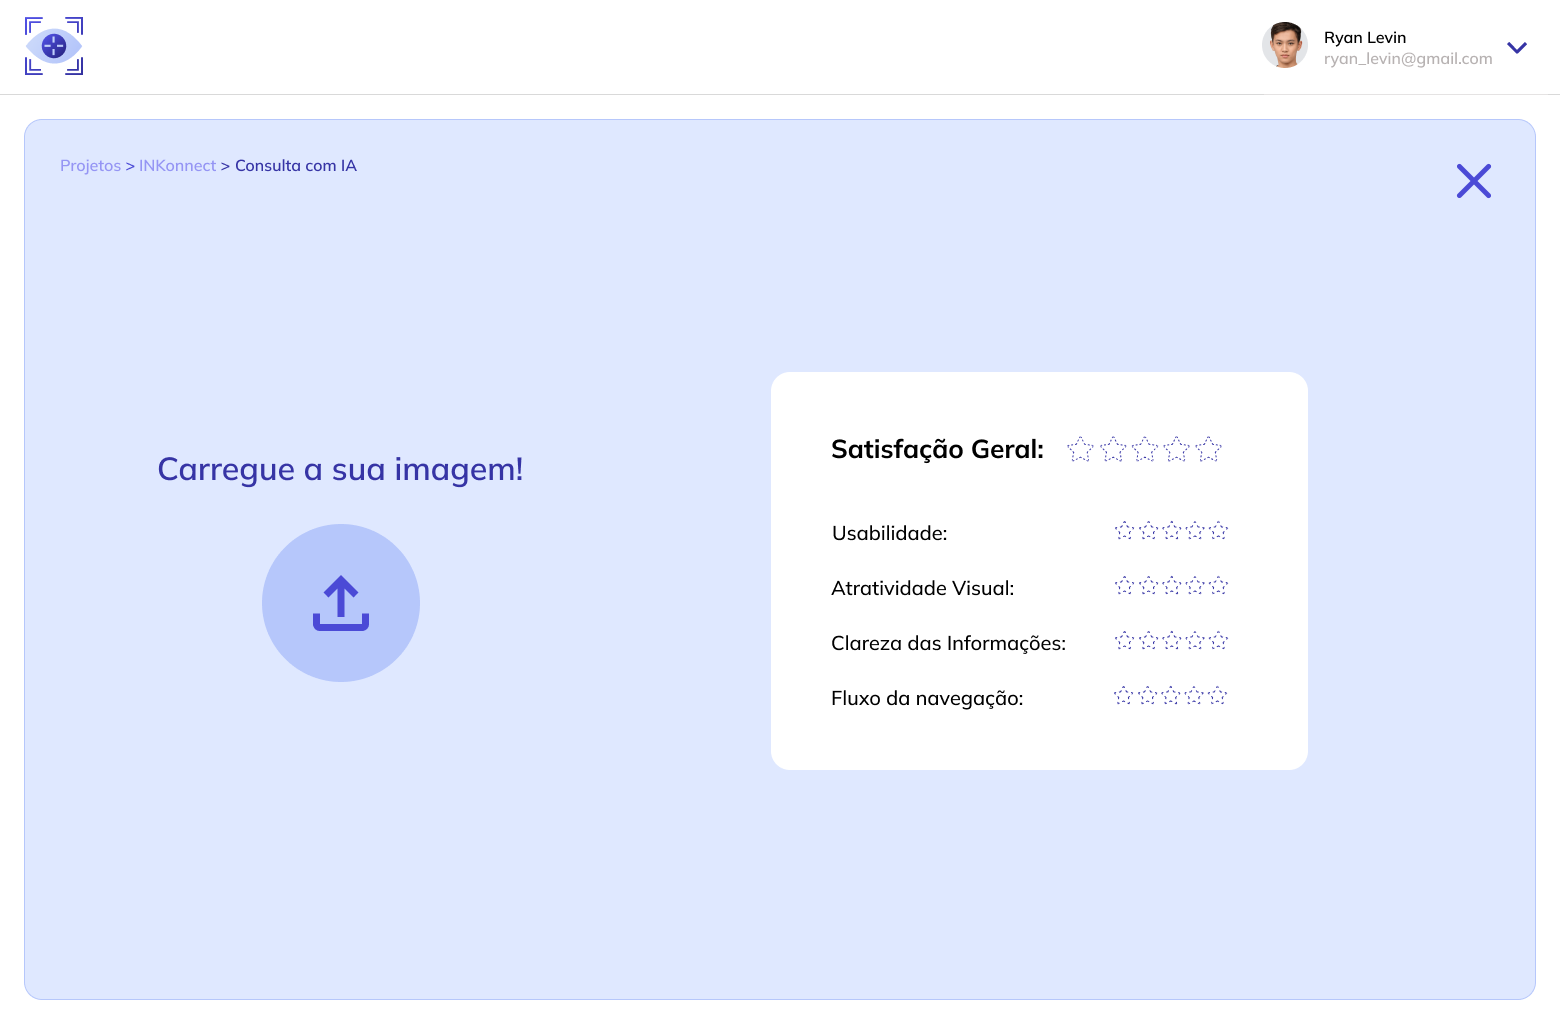
\includegraphics[width=0.72\linewidth]{Illustrations/tela4.png}
    \SourceOrNote{Autoria Própria (2024)}
\end{figure}

A (\Cref{fig:pg-tela5}) ilustra a tela do projeto após receber a avaliação da IA.

\begin{figure}[H]
    \centering
    \caption{Tela 5 - Resposta IA}%
    \label{fig:pg-tela5}
    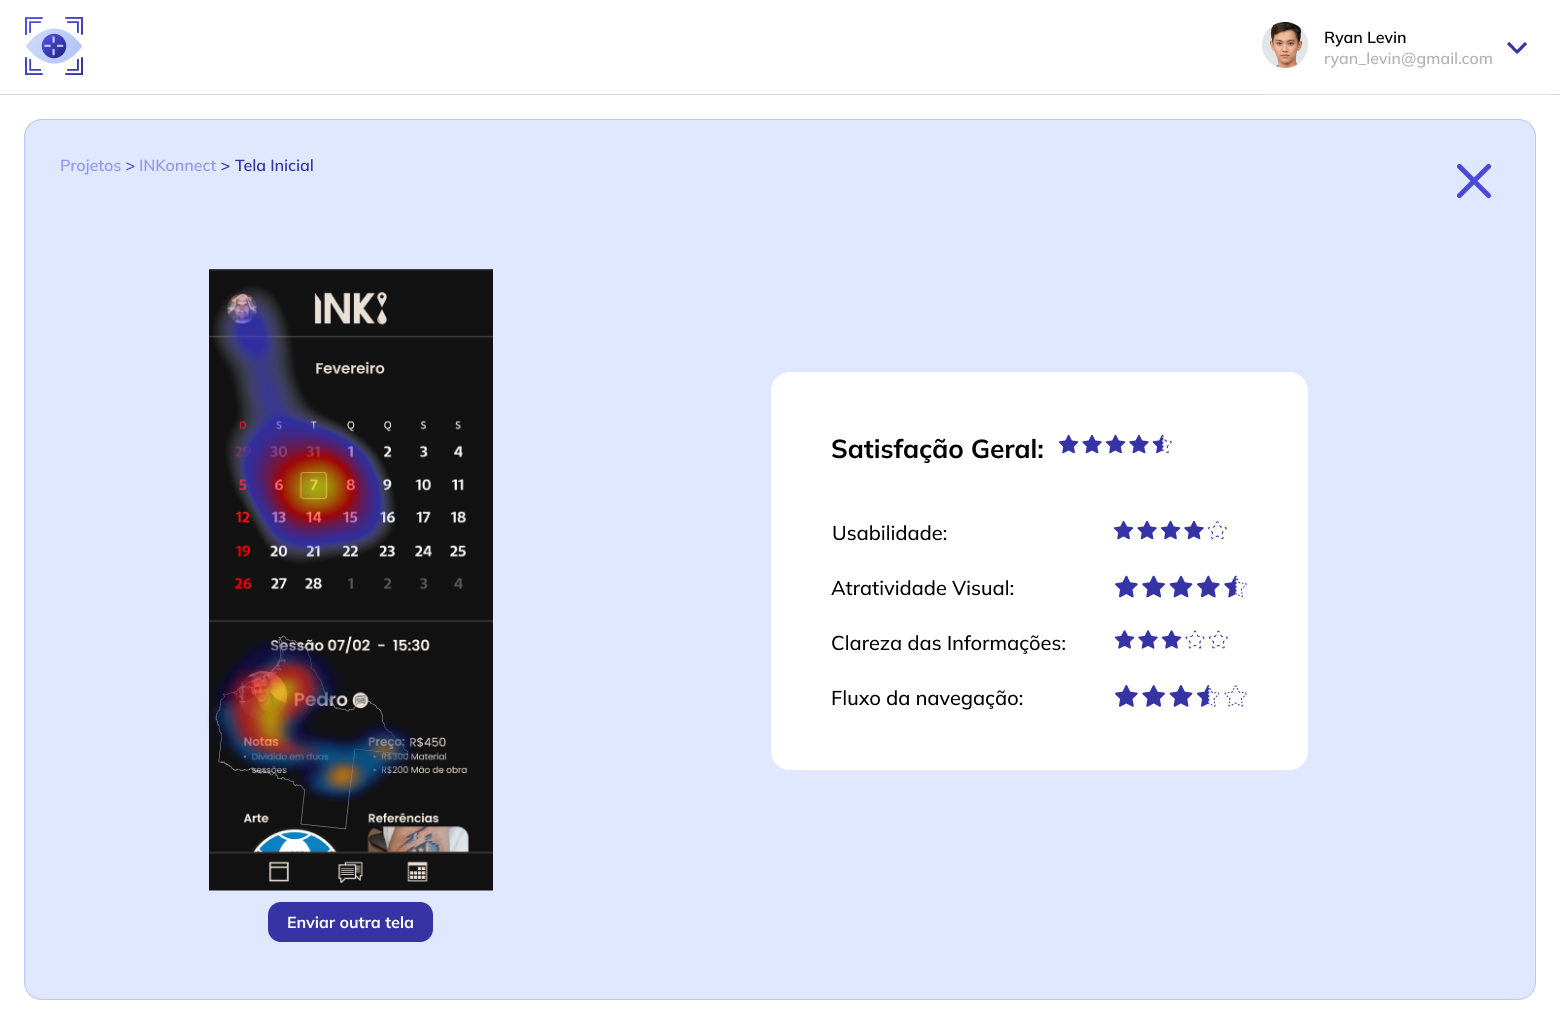
\includegraphics[width=0.72\linewidth]{Illustrations/tela5.png}
    \SourceOrNote{Autoria Própria (2024)}
\end{figure}

Ao selecionar a opção de fazer um novo teste na (\Cref{fig:pg-tela2}), o designer deve colocar as informações pessoais do cliente para iniciar o teste (\Cref{fig:pg-tela6}).

\begin{figure}[H]
    \centering
    \caption{Tela 6 - Registro do cliente}%
    \label{fig:pg-tela6}
    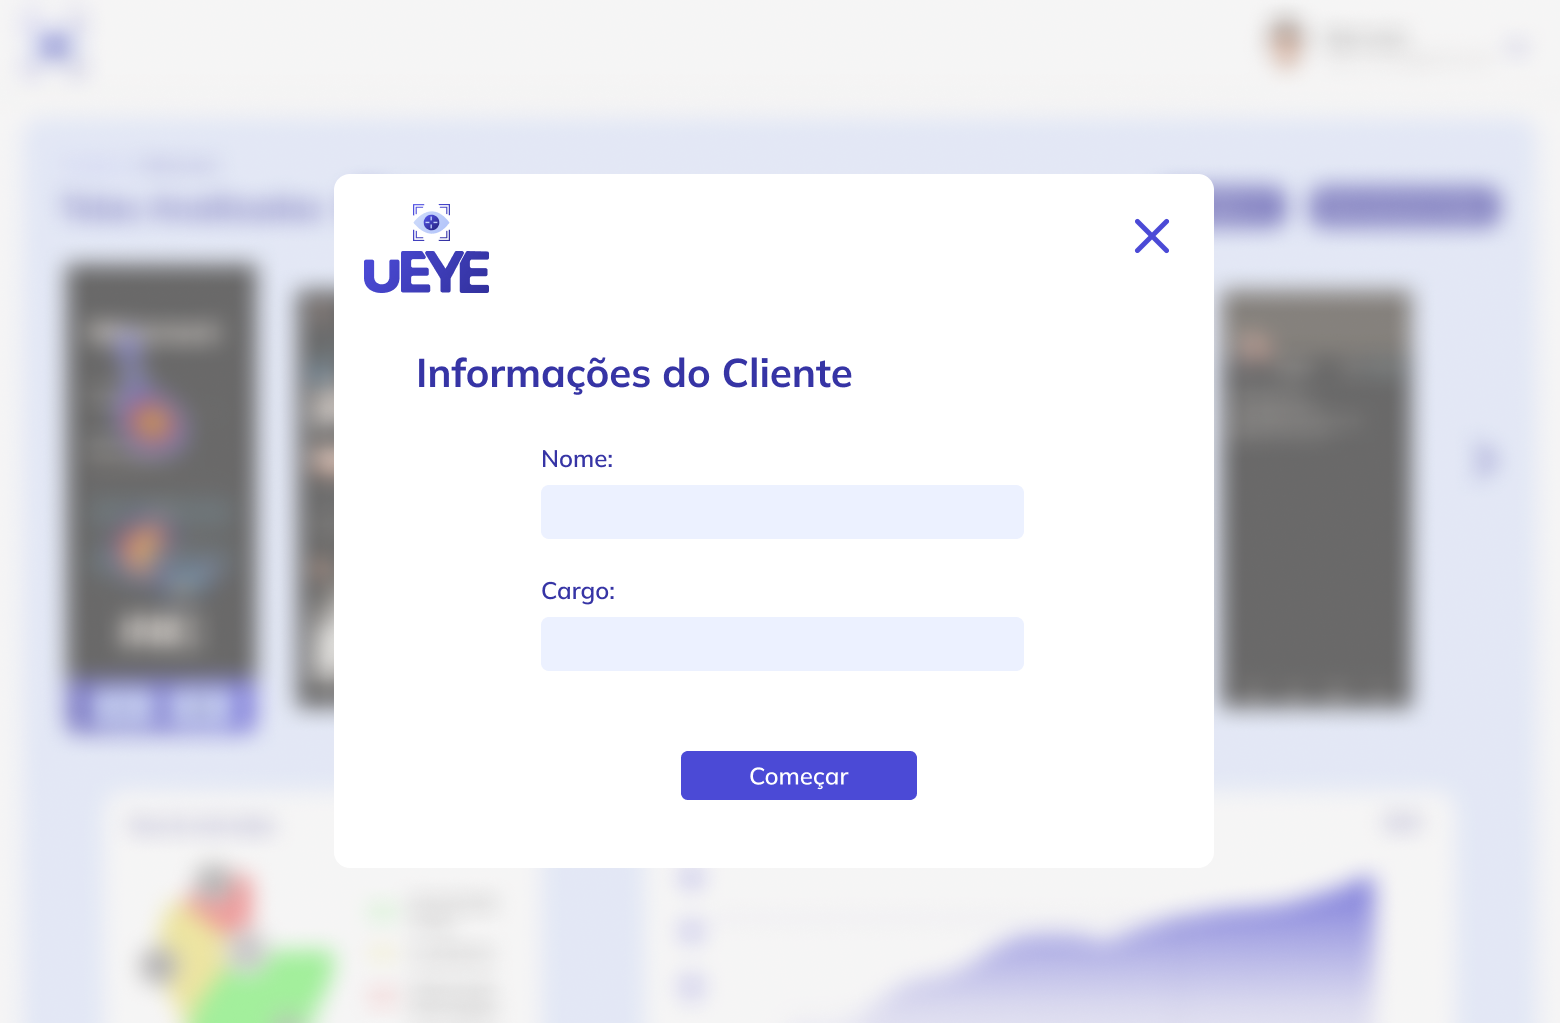
\includegraphics[width=0.72\linewidth]{Illustrations/tela6.png}
    \SourceOrNote{Autoria Própria (2024)}
\end{figure}

A (\Cref{fig:pg-tela7}) ilustra o design sendo exibido ao cliente enquanto ele faz o Eye Tracking.

\begin{figure}[H]
    \centering
    \caption{Tela 7 - Eye Tracking}%
    \label{fig:pg-tela7}
    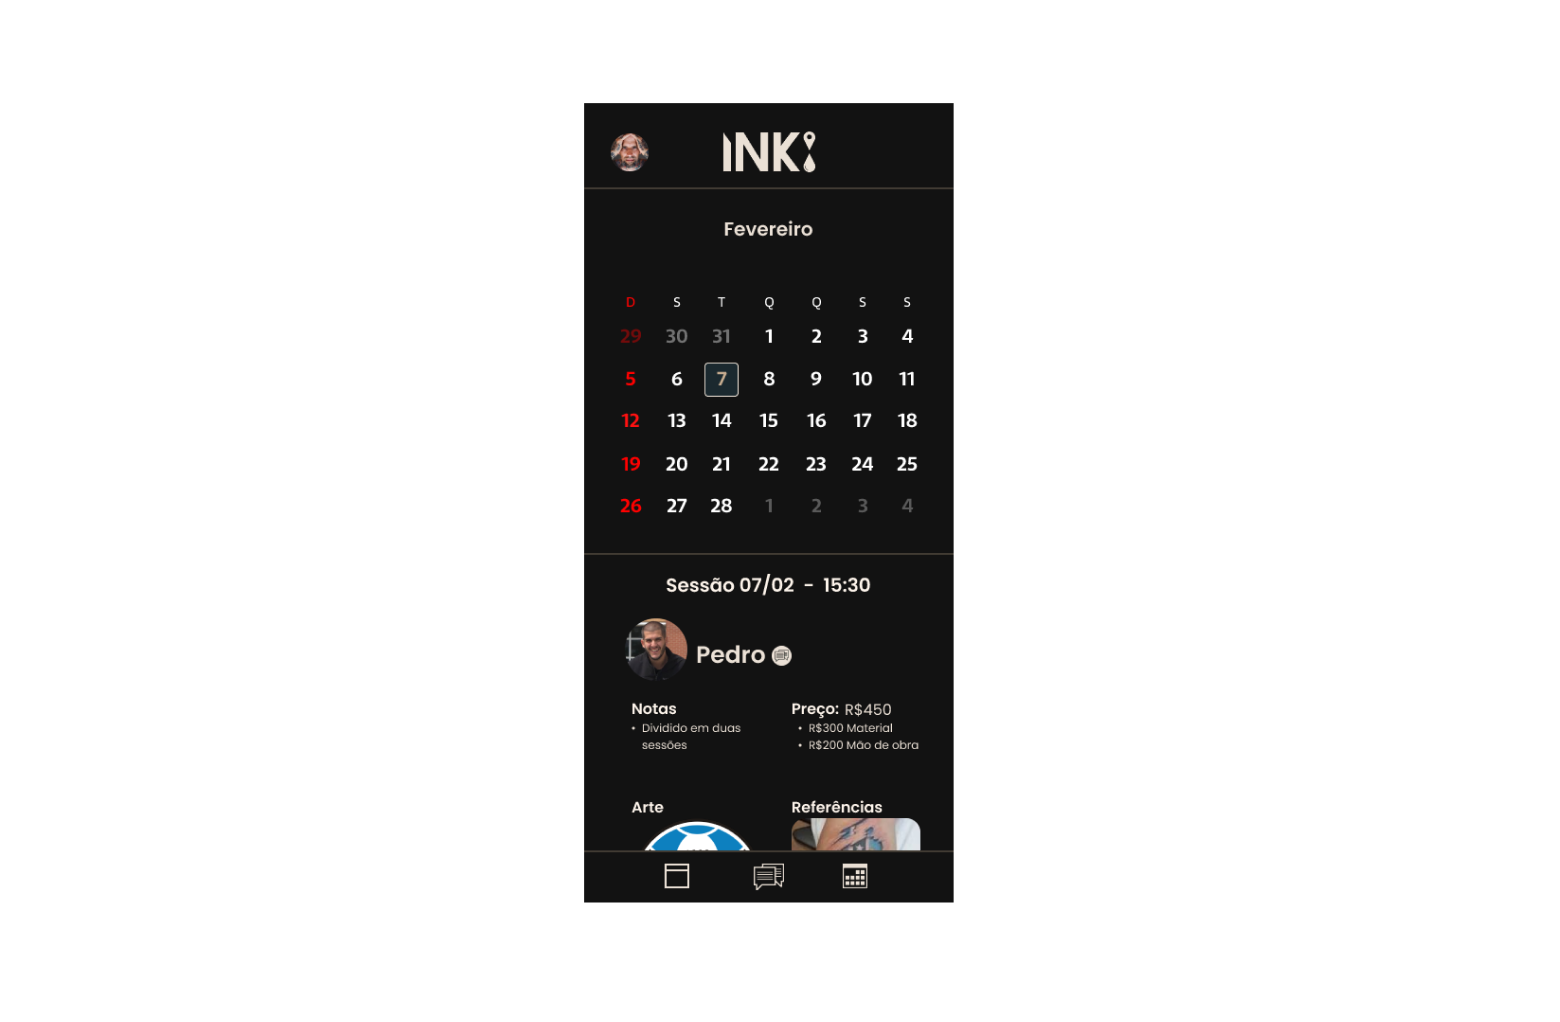
\includegraphics[width=0.72\linewidth]{Illustrations/tela7.png}
    \SourceOrNote{Autoria Própria (2024)}
\end{figure}

Após o teste, a tela (\Cref{fig:pg-tela8}) a seguir será exibida ao cliente para que ele forneça o devido feedback, dados os quais serão utilizados para retroalimentar a IA.

\begin{figure}[H]
    \centering
    \caption{Tela 8 - Formulário de feedback}%
    \label{fig:pg-tela8}
    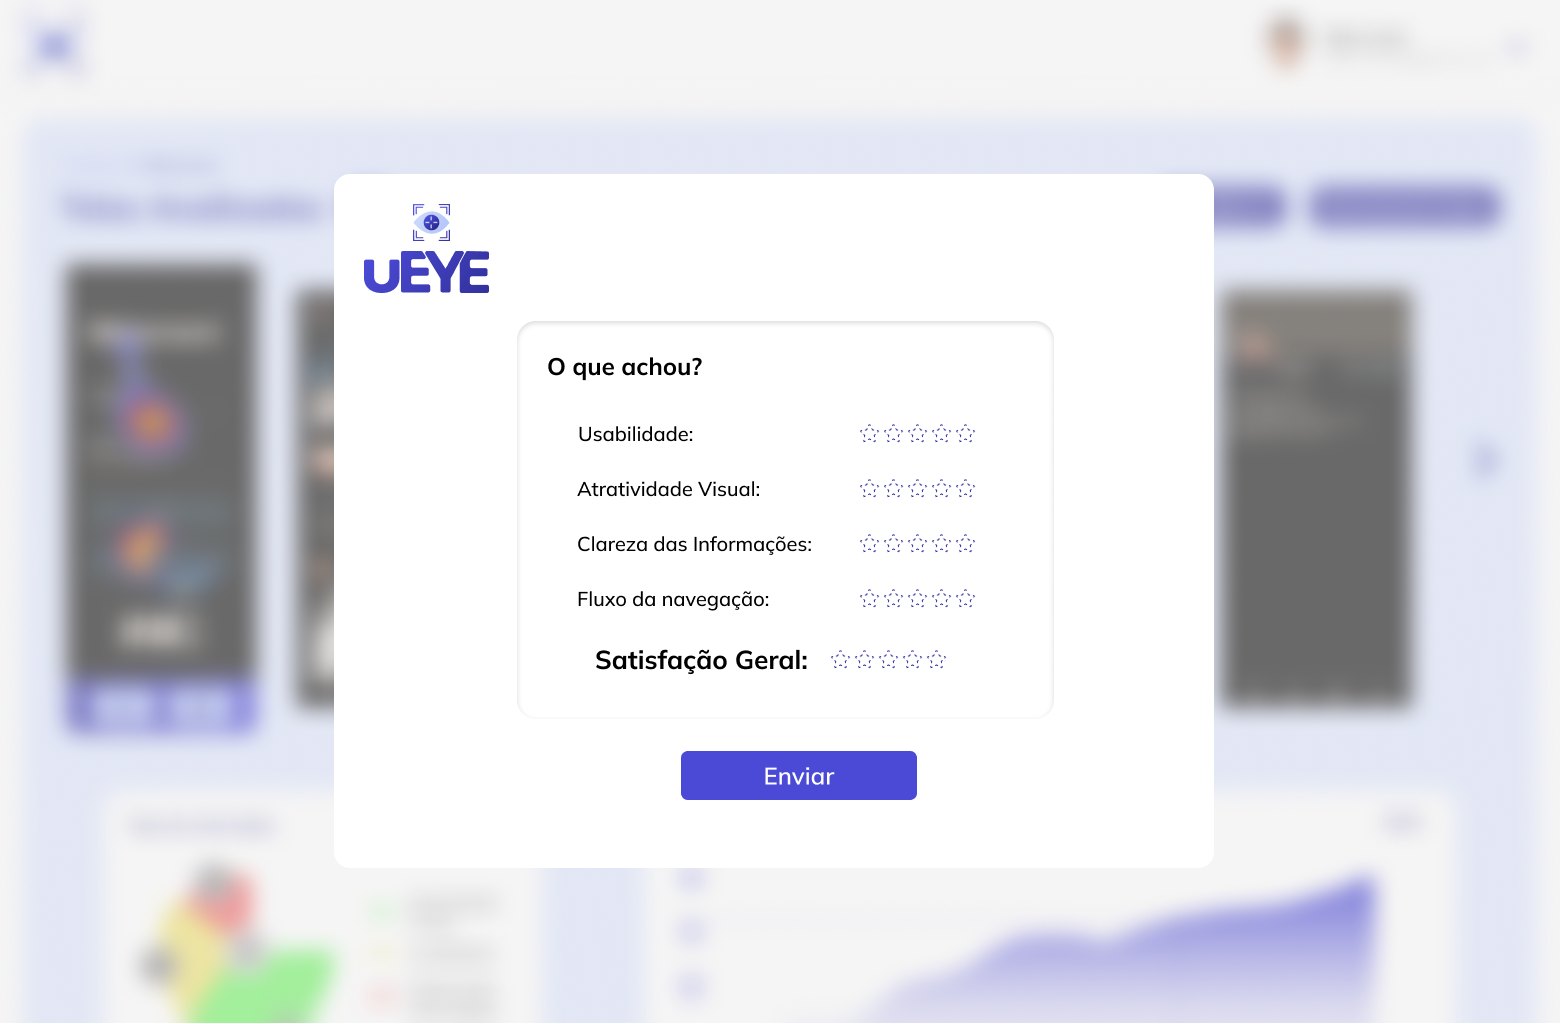
\includegraphics[width=0.72\linewidth]{Illustrations/tela8.png}
    \SourceOrNote{Autoria Própria (2024)}
\end{figure}

Ao selecionar o botão “Ver avaliações” na (\Cref{fig:pg-tela2}), o designer tem acesso ao histórico de avaliações dos clientes, como na imagem a seguir.

\begin{figure}[H]
    \centering
    \caption{Tela 9 - Histórico de avaliações dos clientes}%
    \label{fig:pg-tela9}
    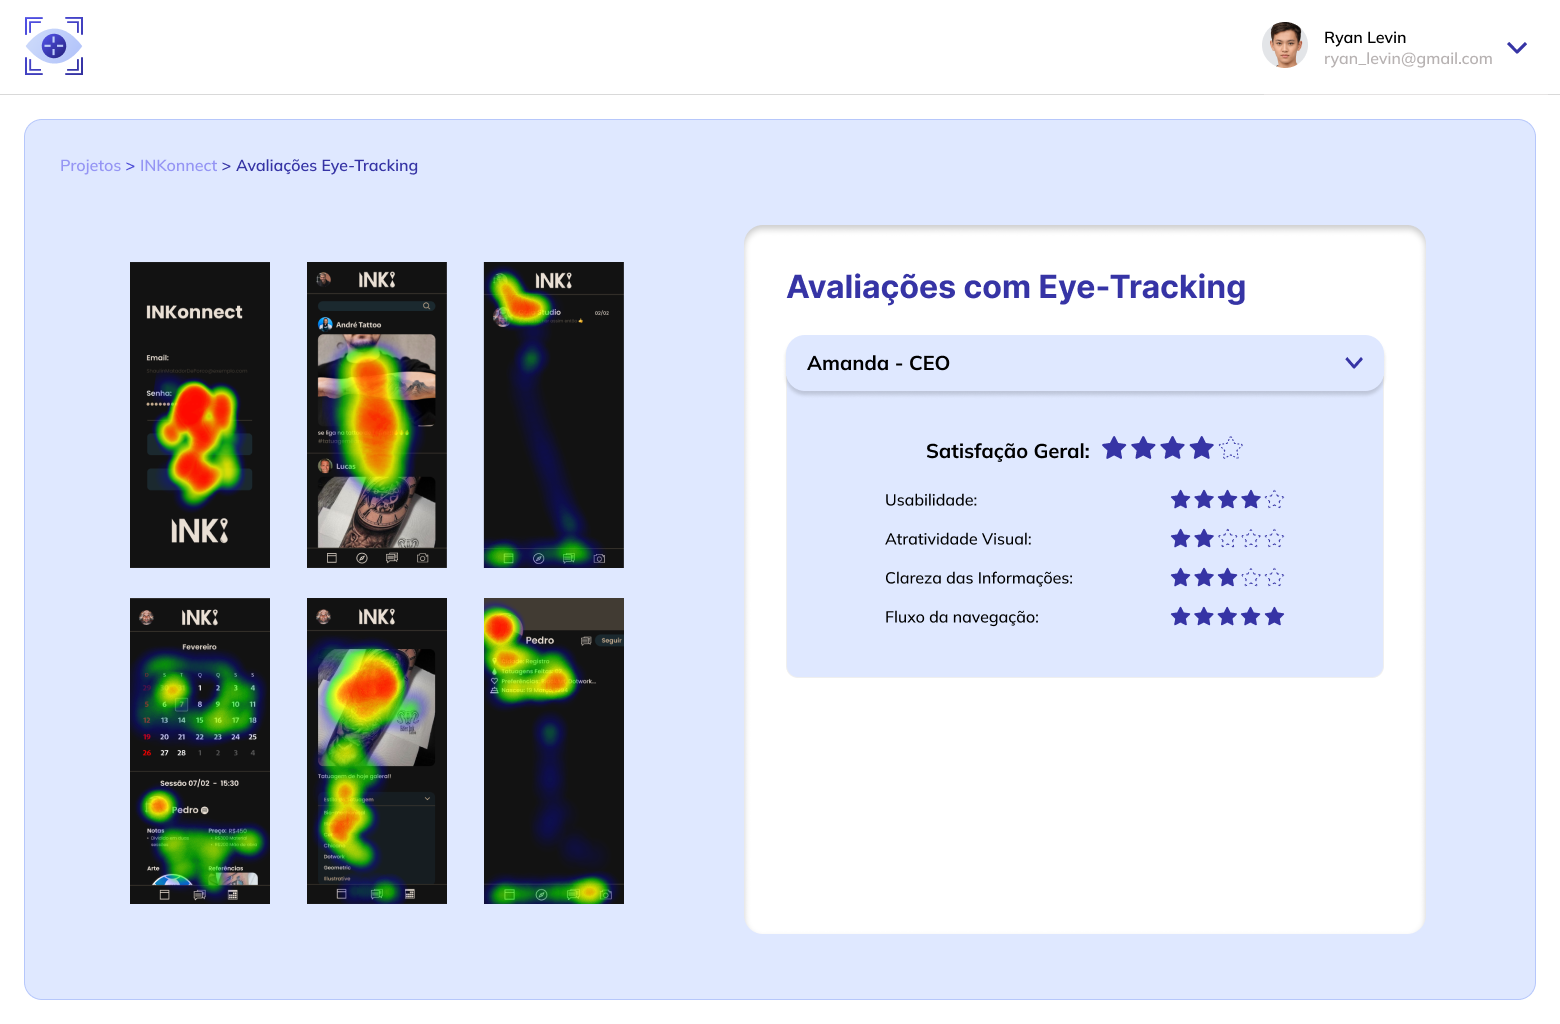
\includegraphics[width=0.72\linewidth]{Illustrations/tela9.png}
    \SourceOrNote{Autoria Própria (2024)}
\end{figure}

\subsection*{MODELO DE NEGÓCIOS}
O desenvolvimento do modelo de negócios para o uEye teve como base a metodologia Business Model Canvas, que oferece uma visão ampla e organizada dos elementos essenciais para a viabilidade do projeto. Este modelo foi escolhido por sua capacidade de sintetizar as principais áreas do negócio, permitindo compreender como o uEye pode gerar valor para os designers de UI/UX, além de mapear os recursos necessários, atividades principais e potenciais fluxos de receita.

O Canvas foi construído a partir de uma análise detalhada das necessidades do público-alvo, segmentado como designers de interfaces interessados em otimizar seus projetos com o auxílio de tecnologias como rastreamento ocular e inteligência artificial. Cada elemento do Canvas reflete decisões tomadas para alinhar a proposta de valor do uEye com as expectativas do mercado e com os recursos disponíveis para o projeto.

\begin{figure}[H]
    \centering
    \caption{Canvas}%
    \label{fig:pg-canvas1}
    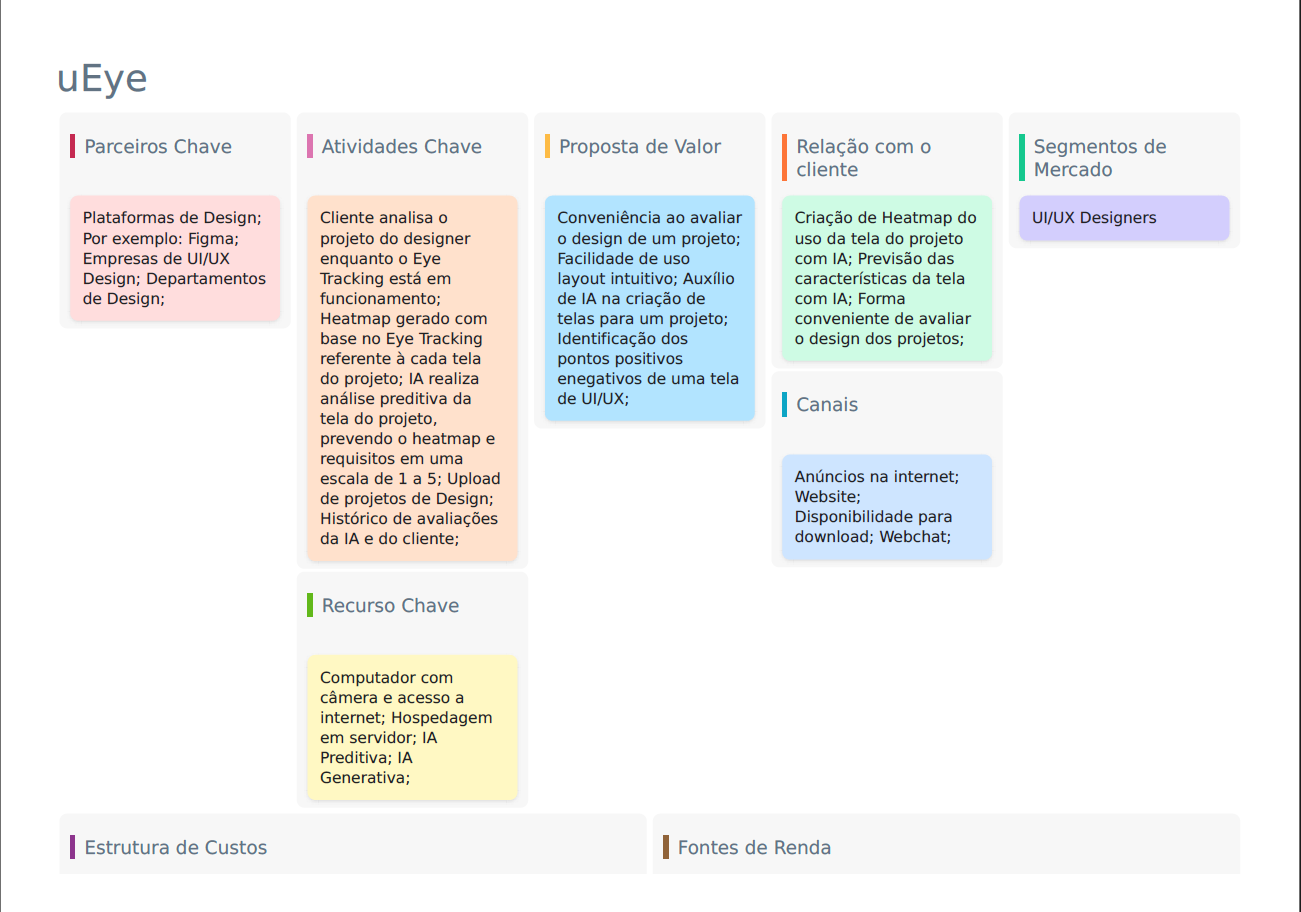
\includegraphics[width=0.72\linewidth]{Illustrations/canvas1.png}
    \SourceOrNote{Autoria Própria (2024)}
\end{figure}

\begin{figure}[H]
    \centering
    \caption{Canvas - Continuação}%
    \label{fig:pg-canvas2}
    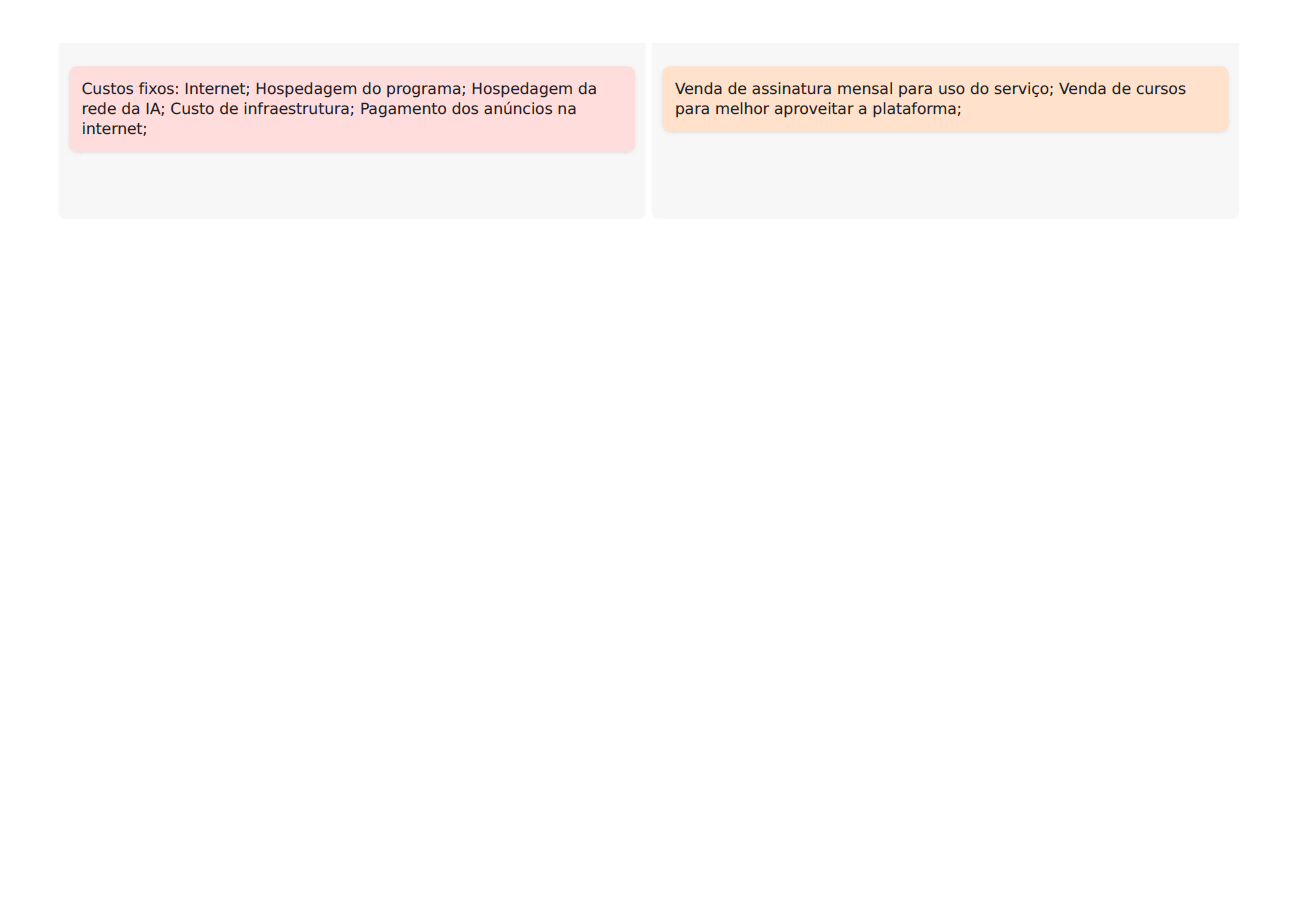
\includegraphics[width=0.72\linewidth]{Illustrations/canvas2.png}
    \SourceOrNote{Autoria Própria (2024)}
\end{figure}

\subsection*{ALGORITMO DE ORDENAÇÃO}
O Merge Sort é um algoritmo de ordenação eficiente baseado na técnica de "dividir para conquistar". Ele divide recursivamente o array original em subarrays menores até que cada um contenha um único elemento, e então realiza a fusão desses subarrays ordenados por meio de um processo denominado merge. A complexidade de tempo do Merge Sort é O(n * log n), o que significa que ele tem uma performance consistente e eficiente, tanto no melhor quanto no pior caso. Essa complexidade é uma das mais eficientes entre os algoritmos de ordenação baseados em comparação. \textcite{Brunet}

A seção de código abaixo apresenta a implementação do algoritmo de ordenação Merge Sort em Python. O Merge Sort foi utilizado para ordenar os dados do heatmap, o que garante que a intensidade do foco visual do usuário seja organizada de forma a facilitar a análise posterior.

\noindent
\textbf{MERGE\_SORT}(arr)\\
\texttt{SE tamanho(arr) > 1 ENTAO}\\
\texttt{    meio = tamanho(arr) \textbackslash 2}\\
\texttt{    esquerda = arr[0 : meio]}\\
\texttt{    direita = arr[meio : tamanho(arr)]}\\
\\
\texttt{    MERGE\_SORT(esquerda)}\\
\texttt{    MERGE\_SORT(direita)}\\
\\
\texttt{    i = 0}\\
\texttt{    j = 0}\\
\texttt{    k = 0}\\
\\
\texttt{    ENQUANTO i < tamanho(esquerda) E j < tamanho(direita) FACA}\\
\texttt{        SE esquerda[i] < direita[j] ENTAO}\\
\texttt{            arr[k] = esquerda[i]}\\
\texttt{            i = i + 1}\\
\texttt{        SENAO}\\
\texttt{            arr[k] \textbackslash leftarrow direita[j]}\\
\texttt{            j = j + 1}\\
\texttt{        FIM SE}\\
\texttt{        k = k + 1}\\
\texttt{    FIM ENQUANTO}\\
\\
\texttt{    ENQUANTO i < tamanho(esquerda) FACA}\\
\texttt{        arr[k] = esquerda[i]}\\
\texttt{        i = i + 1}\\
\texttt{        k = k + 1}\\
\texttt{    FIM ENQUANTO}\\
\\
\texttt{    ENQUANTO j < tamanho(direita) FACA}\\
\texttt{        arr[k] = direita[j]}\\
\texttt{        j = j + 1}\\
\texttt{        k = k + 1}\\
\texttt{    FIM ENQUANTO}\\
\texttt{FIM SE}

As figuras a seguir ilustram a matriz de rastreamento ocular, que armazena valores correspondentes ao tempo de foco do usuário. A primeira figura apresenta a matriz gerada antes da aplicação do algoritmo Merge Sort, enquanto a segunda mostra a matriz após a ordenação dos valores utilizando o Merge Sort.

\begin{figure}[H]
    \centering
    \caption{Matrzi de rastreamento ocular não ordenada}%
    \label{fig:pg-mergesort}
    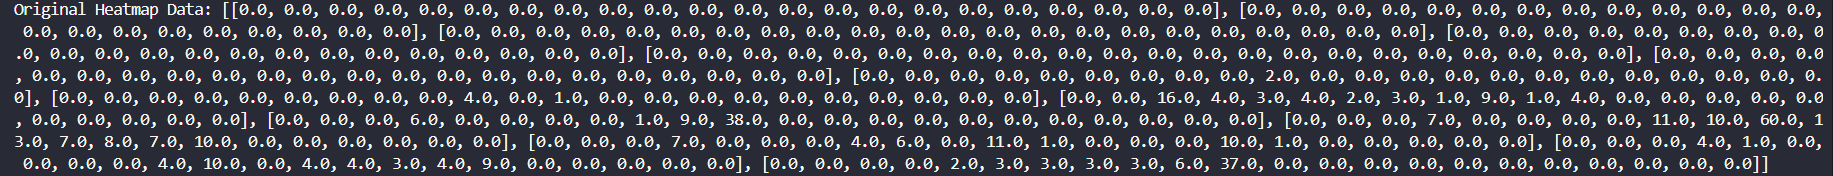
\includegraphics[width=0.72\linewidth]{Illustrations/desordenado.png}
    \SourceOrNote{Autoria Própria (2024)}
\end{figure}

\begin{figure}[H]
    \centering
    \caption{Matrzi de rastreamento ocular ordenada}%
    \label{fig:pg-mergesort2}
    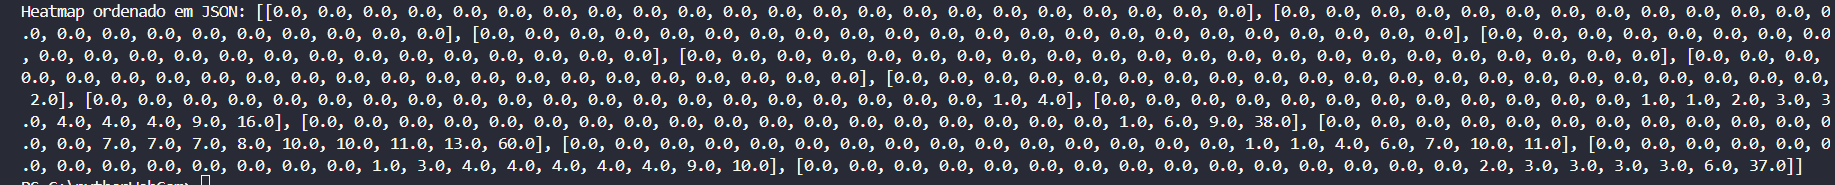
\includegraphics[width=0.72\linewidth]{Illustrations/ordenado.png}
    \SourceOrNote{Autoria Própria (2024)}
\end{figure}


A análise assintótica do Merge Sort visa entender seu comportamento em termos de tempo e espaço à medida que o tamanho da entrada cresce. A seguir, é apresentado um desdobramento do algoritmo para explicar como ele pode ser descrito por meio de uma equação de recursão.

\begin{itemize}
    \item Divisão: O algoritmo divide o array original em duas metades. Esse processo de divisão implica em uma operação constante de cálculo do meio do array e criação dos subarrays.
    \item Recursão: Após a divisão, o algoritmo chama a si mesmo recursivamente para ordenar os subarrays. Cada chamada recursiva trabalha em um subarray de tamanho \( \frac{n}{2} \).
    \item Merge: Após ordenar os subarrays, o Merge Sort realiza o processo de merge, no qual os subarrays ordenados são combinados. O merge compara os elementos dos subarrays e os coloca em ordem, o que exige \( n \) operações.
\end{itemize}

A equação de recursão que descreve o funcionamento do Merge Sort é dada por:

\[
\text{merge-sort}(n) = 
\begin{cases} 
1 & \text{se } n = 1 \\
14 \times \left( 2 \times \text{merge-sort}\left(\frac{n}{2}\right) \right) + n & \text{se } n > 1
\end{cases}
\]

Na análise assintótica do Merge Sort, o caso base ocorre quando o tamanho do array é igual a 1, e o algoritmo não realiza operações além de retornar. Quando \( n > 1 \), o algoritmo realiza duas chamadas recursivas (uma para o subarray esquerdo e outra para o subarray direito), cada uma lidando com um array de tamanho \( \frac{n}{2} \). Além disso, o processo de merge entre os subarrays exige \( n \) operações.

O fator 14 refere-se ao número de linhas da matriz em que o algoritmo é executado, representando a dimensão do problema em um contexto específico. Em termos práticos, isso significa que o Merge Sort realiza suas operações de divisão, recursão e mesclagem em cada uma dessas 14 linhas, impactando diretamente o custo computacional total do algoritmo.